% !TEX root = Technologierecherche.tex
\section{Greifer}
\subsection{mechanisch}
Greifer besteht aus einer festen Seite und einer beweglichen Seite

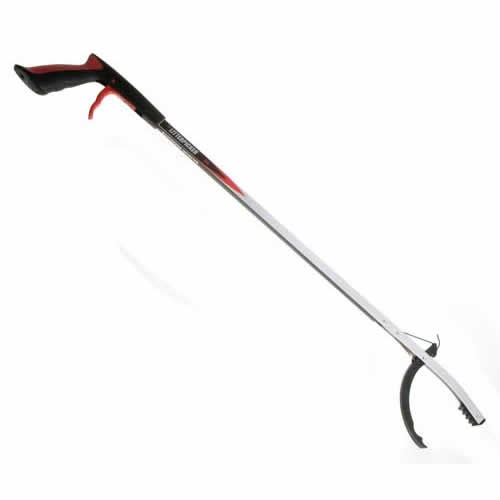
\includegraphics[width=0.5\textwidth]{Images/Gripper6.png}

Eigenschaften: 
\begin{itemize}
\item sehr einfacher Aufbau
\item wenige Teile notwendig
\item nicht präzise Lösung
\end{itemize}

Greifer mittels 2 Zahnräder gleichmässig schliessen

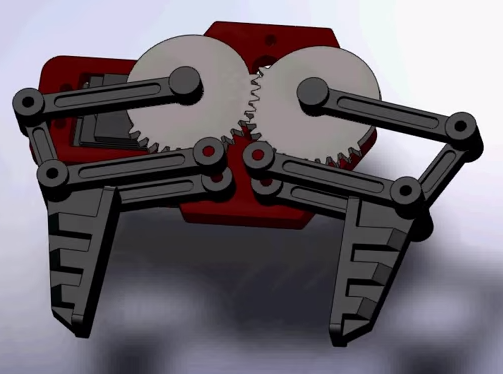
\includegraphics[width=0.5\textwidth]{Images/Gripper2.png}

Eigenschaften:
\begin{itemize}
\item präzise Lösung
\item aufwändiger Aufbau
\item symmetrischer Aufbau
\end{itemize}

\subsection{pneumatisch}
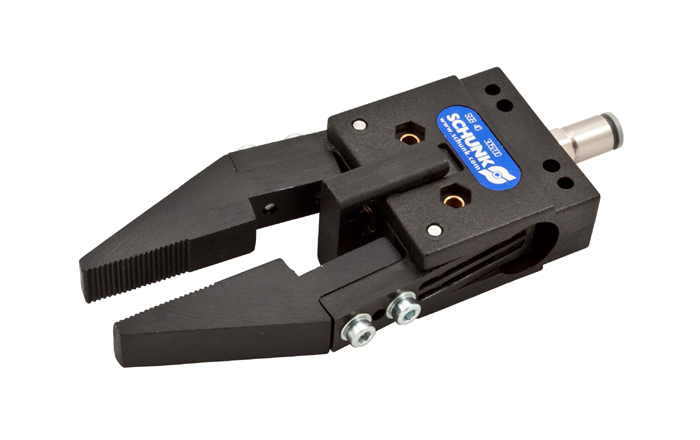
\includegraphics[width=0.5\textwidth]{Images/pneumatGr_schunk.jpg}

Eigenschaften: 
\begin{itemize}
\item Druckluft-Aggregat notwendig
\item hohe Präzision
\item teuer
\end{itemize}

\subsection{magnetisch}
Greifen der M4 Schrauben und Muttern mittels eines Elektromagneten

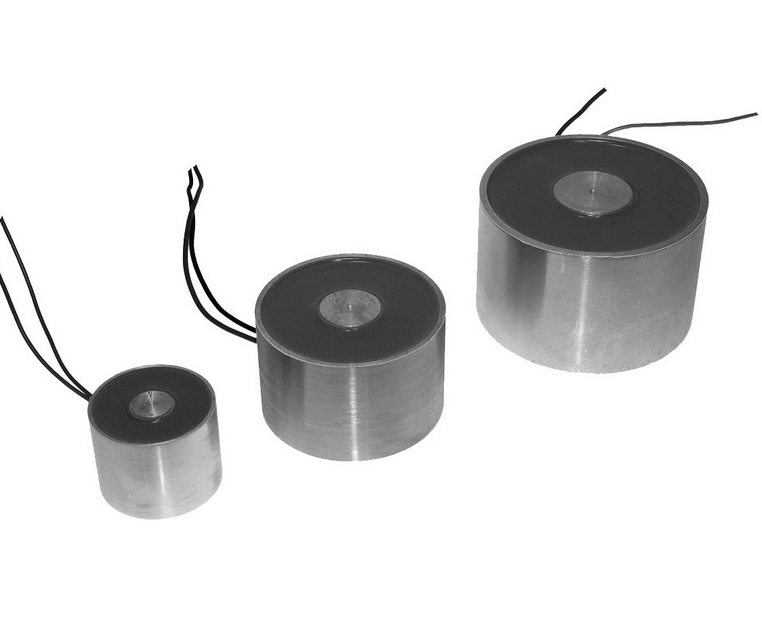
\includegraphics[width=0.5\textwidth]{Images/Magnetgreifer.png}

Eigenschaften:
\begin{itemize}
\item einfacher Aufbau
\item einfache Integration
\item fraglich ob genügend stark
\end{itemize}